
\chapter{Seminario 1: \textit{Data and AI Law}}
Tenuto dal Co-founder e CEO di ICC Digital Media 1999, Giuseppe Fragola, in data 28 Novembre 2025.

\section{L'importanza dei dati - segreti industriali}
Qualsiasi rivoluzione tecnologica ha a che fare con i dati. I dati sono il comune denominatore di ogni settore. I dati non sono da vedersi solo come dati del singolo, ma anche informazioni strategiche e  segreti industriali, tra cui:

\begin{multicols}{2}
	\begin{itemize}
		\item Formule
		\item Progetti
		\item Fornitori e prezzi
		\item Organizzazione
		\item Produzione
		\item Tecnologie in uso
	\end{itemize}
\end{multicols}

A tutela dei dati relativi ai segreti industriali, nasce un ampio corpus informativo.

\subsection{Data Is The New Oil}
\textbf{I dati hanno una valenza strategica enorme}.
Le organizzazioni criminali, tramite attacchi hacker, puntano a ottenere informazioni preziose per fare speculazione economica. Tra questi dati, ci sono \textbf{brevetti}, \textbf{bilanci}, \textbf{fornitori} e \textbf{contratti}. Inoltre, visto l'inevitabile crescita della quantità di dati, i crimini informatici relativi al loro ottenimento illecito, sono destinati ad aumentare nel tempo. 

\subsection{\textit{Mission Genesis} - 25 Novembre 2025}
Donald Trump ha recentemente firmato un ordine esecutivo per condividere i dati scientifici di tutte le agenzie governative e utilizzare l'AI (creando un \textit{data lake}\footnote{Un data lake è un
	repository centralizzato che archivia grandi quantità di dati strutturati, semi-strutturati e non strutturati nel loro formato nativo. A differenza di un data warehouse, i dati vengono archiviati senza una struttura predefinita, il che consente una maggiore flessibilità per diverse analisi, tra cui Big Data, machine learning e analisi in tempo reale.}) per accelerare ricerca, sicurezza nazionale e la razionalizzazione la rete elettrica nazionale.

\subsection{Norme: Data Protection e Copyright}
Lavorare con i dati, costringe qualsiasi operatore coinvolto a confrontarsi con le norme relative alla data protection e al diritto d'autore.

\section{Data Protection}
Iniziamo \textbf{distinguendo privacy} dalla \textbf{data protection}. La privacy è infatti il diritto alla riservatezza nella propria sfera privata da parte di terzi (\textit{Right to be alone}). La data protection fa invece riferimetno al \textbf{trattamento dei dati personali solo con previa autorizzazione dell'interessato}. I dati possono essere trattati solo col consenso di hi li produce.

\paragraph{Cos'è un dato personale?} Una qualsiasi \textbf{informazione} che direttamente o indirettamente consente di \textbf{identificare una persona fisica}, o le sue abitudini, lo stile di vita, le relazioni personali, lo stato di salute o lo stato economico.

\subsection{GDPR - La rivoluzione}
L'Europa decide di tutelare i propri cittadini, con obiettivo ultimo una bolla di protezione relativa ai dati personali. Nasce il regolamento GDPR. Questo, si applica a:
\begin{itemize}
	\item Coloro che avendo sede EU trattano dati di soggetti interessati \textbf{a prescindere dalla loro nazionalità} o \textbf{residenza}.
	\item Coloro non EU che per la vendita di beni o servizi, \textbf{trattano dati personali} di soggetti interessati \textbf{che si trovano in EU}.
\end{itemize}

Gli spunti sono i seguenti:
\begin{itemize}
	\item\textbf{Privacy by Design}: ogni applicazione che tratta dati degli utenti, deve nascere privacy-oriented, concepito e sviluppato avendo in mente la loro tutela.
	\item\textbf{Privacy by Default}: tutte le opzioni per rispettare la privacy devono essere di default.
	\item\textbf{Consent}
	\item\textbf{Portabilità}
	\item\textbf{Data Breach Notification}, obbligata dopo qualsiasi data breach. La norma non da degli obblighi di sicurezza, ma sei responsabile di qualsiasi conseguenza.	
\end{itemize}

\noindent
ma tra i quelli più rivoluzionari, abbiamo anche:
\begin{itemize}
	\item \textbf{Minimizzazione}: ogni azienda deve acquisire il minimo indispensabile dei dati rispetto alla finalità per le quali solo trattati. Registrarsi una newsletter dovrebbe consentire solo all'acquisizione dell'e-mail, non del numero di telefono o altri dati sensibili. Questo implica anche la possibilità, da parte dell'utente, di eliminare account personali su piattaforme online.
	\item \textbf{Informativa e Consenso granulare}: il consenso deve essere rilasciato specificamente per \textbf{ciascuna delle finalità di trattamento} dichiarate, \textbf{una ad una}.
	
	\item \textbf{Temporaneità}: i dati devono avere tempo di vita limitato, non possono 
\end{itemize}

Le sanzioni previste arrivano fino al $4\%$ del \textbf{fatturato del consolidato mondiale del gruppo}.

\subsection{Sui Cookies}
Conosciamo già i cookies: questi permettono di tracciare informazioni sul browser dell'utente (cookies di sessione e persistenti). Tra questi, abbiamo cookies di prime parti e di terze parti.

\begin{itemize}
	\item I cookies di prime parti sono generati e leggibili solo dal dominio chi li ha creati
	\item I cookies di terze parti sono creati da domini esterni a quello che si sta visitando. Questo permette facilmente di tracciare informazioni sulle abitudini di un utente, ottenendo dati (o almeno, del suo browser).
\end{itemize}

\paragraph{Direttiva del 2009 sui Cookies} l'UE introduce la direttiva nota come "Cookies Directive" per regolamentare l'uso dei cookie online. L'obiettivo della norma è quello di \textbf{garantire informazione chiara} agli utenti e \textbf{regolamentare l'uso dei cookie} attraverso \textbf{obbligo di informativa} e \textbf{invio solo previo consenso}.

\section{Copyright e diritto d'autore}

Disambiguiamo i termini.
\begin{itemize}
	\item Il \textbf{copyright} è il diritto di copia. Io che ho creato un contenuto, ho diritto ad una \textit{fee}, un rimborso, ogni qual volta in cui qualcuno me ne richieda una copia. Dura all'incirca 50 anni.
	\item Il \textbf{diritto d'autore} tutela l'autore e la paternità dell'opera, e si acquisisce con la creazione dell'opera stessa. Dura 70 anni dalla morte dell'autore.
\end{itemize}

\subsection{Diritto d'autore}
Riconosce dei \textbf{diritti morali indisponibili}. Tra questi abbiamo che sono \textbf{indisponibili}, sono riconosciuti a priori. Si ha il diritto a \textbf{paternità}, \textbf{integrità}, \textbf{inedito}, \textbf{pentimento}. I diritti patrimoniali sono invece disponibili, e sono diritto di \textbf{riproduzione}, \textbf{diffusione}, \textbf{modifica} e \textbf{traduzione}.

Nonostante la durata fissata sia 70 anni dalla morte dell'autore, esistono delle durate particolari sono quelle di opere a \textbf{contributo indistinguibile} e \textbf{opere collettive}.

\subsection{Alla tutela del Software}
Dopo anni di incertezza normativa, il software p stato inserito tra le \textbf{opere dell'ingegno} tutelate dalla legge sul \textbf{diritto d'autore}. la tutela riguarda esclusivamente la forma espressiva originale del software (codice), ma non l'idea, che può essere riprodotta mediante un codice diverso. Allo sviluppatore spettano:

\begin{itemize}
	\item \textbf{Diritti morali} - parternità indisponibile
	\item \textbf{Diritti patrimoniali} - riproduzione, traduzione, adattamento, trasformazione, distribuzione
\end{itemize}

questi, sono però cedibili (a tempo determinato o indeterminato) mediante opportune licenze d'uso. \textit{Consiglio: non perdere mai le licenze ai software! Tieni sempre una cartella con le licenze.}

\subsubsection{Comprare il software o una licenza?}
Ogni qual volta che "compriamo" un software, in realtà noi stiamo acquistando una licenza (temporanea o non). Comprare un software, in senso stretto, significherebbe acquisirne il sorgente.

\subsubsection{Principio d'esaurimento}
Ogni volta che un bene viene immesso nel mercato, chi li immette nel mercato non ha più controllo delle eventuali rivendite e della libera circolazione.

\section{AI e Copyright}
Tra i punti più caldi relativi all'intelligenza artificiale e il Copyright, abbiamo:

\begin{itemize}
	\item AI e creazione di opere nuove.
	\item AI e creazione di opere derivate.
	\item AI e i dati d'addestramento.
\end{itemize}

\begin{center}
	\textit{A chi appartengono i diritti d'autore in questi casi?}
\end{center}


\subsubsection{Parentesi sulle AI generative}
L'AI generativa è una categoria di AI che permette la generazione di testi, immagini, video e codice grazie a modelli di machine learning supervisionati, reinforcement learning e LLM addestrati su quantità di dati sempre crescenti. Nel 2022 avviene la prima generazione di contenuti creativi nuovi a partire da un algoritmo. 
\textbf{Le opere generate da AI possono essere tutelate da diritto d'autore?}
Se presentano originalità e creatività al pari di quella umana, questa potrebbe essere tutelata.

\subsection{Posizioni dell'US Copyright Office}
\begin{itemize}
	\item 2023 - Rigetto della richiesta di copuright su un'opera creata da AI. \textit{Non sussiste il necessario nesso tra autore umano ed espressione creativa}.
	\item 2024 - conferma e chiarimento.\textit{ È esclusa ogni tutela per opere create dalla macchina in assenza di una prevalente creatività umana}.
	\item Nodo aperto: \textit{un nodo abbastanza dettagliato è un apporto creativo prevalentemente umano?} \\
	Il tribunale cinese conferma i diritti riconosciuti all'umano, per gli US la questione rimane aperta.
\end{itemize}

\subsection{In Italia}
Se prevale l'apporto creativo umano, l'opera resta un'opera dell'ingegno e gode della piena tutela del diritto d'autore e delle cateogrie IPR tradizionali, attribuite alla persona fisica.
\textit{\textbf{Trattasi di un opera dell'ingegno solo se prevale la creatività umana}}. Un'enorme area grigia giuridica.

\subsection{\textit{Un primo passo }- In Sud Africa}
Il Sud Africa cambia la storia riconoscendo il \textbf{primo brevetto per una invenzione autonomamente creata da una AI}.

\subsection{AI e soggettività giuridica}
Riconoscere una soggettività giuridica a un'AI risolverebbe problemi di attribuzione del diritto e della responsabilità per danno, ma aprirebbe scenari economici e sociali imprevedibili. Il timore riguarda \textbf{AI senzienti e dotate di soggettività}, e il rischio che queste possano diventare \textbf{entità potentissime} e ricchissime.

\subsection{Caso OpenAI}
OpenAI attribuisce agli utenti i diritti sulle opere create, riservandosi il diritto di usare l'immagine generata per il training.

\subsubsection{In assenza di disciplina pattizia}
Se l'utente ha fornito un prompt articolato con dati molto specifici e qualificati, l'umano prevale. Altrimenti, il diritto è da attribuirsi agli sviluppatori dell'AI.

\section{AI e opere derivate}
\begin{center}
	\textit{Chi è il responsabile se un'opera realizzata da AI plagia un'opera altrui?}
\end{center}

Si rimane in attesa di una nuova proposta normativa. Si è valutato di attribuire la responsabilità agli sviluppatori, ma è ancora una questione aperta (e attualmente sospesa).

\section{AIG e addestramento}
I dataset contengono dati appartenenti a qualcuno: anche qui dovrebbe subentrare il diritto d'autore. Incontriamo una serie di problemi. Tra queste, le pubblicazioni e i contenuti scritti pre-AI generativa non hanno valutato come gestire un arrivo del genere. Le principali criticità legali sono
\begin{itemize}
	\item \textbf{Violazione del diritto d'autore} per i dati usati nel training.
	\item \textbf{I dataset pubblici non forniscono indicazioni sull'uso relativo all'AI}.
	\item \textbf{Opere derivate}. Opere troppo simili potrebbero considerarsi plagio.
\end{itemize}
Si conclude che, in molti casi, il problema del DDA non è l'AI, ma sono i dataset.

\subsection{Caso New York Times e OpenAI}
New York Times ha fatto causa a OpenAI e Microsoft per violazione del copyright, accusando le aziende di aver utilizzato milioni di suoi articoli per addestrare i loro modelli di intelligenza artificiale senza autorizzazione o compenso. La causa, intentata nel dicembre 2023, è un punto di riferimento globale sul futuro del diritto d'autore nell'era dell'IA generativa. 

\subsection{FIEG contro Google AI}
Google AI Overview rappresenta un \textit{Traffic Killer}, ossia una criticità per il fatturato delle testate giornalistiche. FIEG sollecità l'AGCM affinche sensibilizzi la Commissione Europea ad aprire un procedimento ai sensi del \textbf{Digital Service ACT}.

\section{AI Act}
È una norma potente che nasce dopo 8 anni di elaborazione, proprio per la complessità della materia. L'obiettivo è stato quello di creare una bolla di AI sicura che garantisca i diritti fondamentali dei cittadini Europei dall'invasione di intelligenze artificiali sviluppate in Cina e negli USA. La norma, purtroppo, nella sua enorme complessità, nasce orfana già dalla sua promulgazione: nei giorni adiacenti alla sua redazione, viene rilasciatala prima AI generativa, creando una norma stroncata, incompleta. Riesce tuttavia a tutelare i cittadini dal profiling invasivo, e a tutelare il diritto d'autore.

\section{AI Risk Piramid}
Il legislatore è consapevole di non poter creare delle categorie di intelligenze artificiali: definisce quindi una \textbf{piramide del rischio}, categorizzando ciascuna AI (attuale e futura) in opportuni livelli di questa piramide, in funzione del rischio che questa rappresenta per l'umanità. Ciascuna di queste categorie, rappresenta degli obblighi molto particolari.

\begin{figure}[tbph]
	\centering
	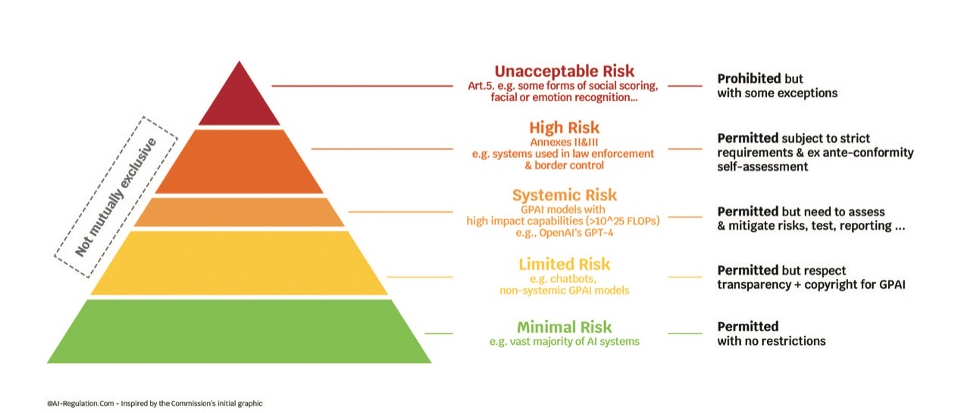
\includegraphics[width=1\linewidth]{images/risk-pyramid}
\end{figure}


Questa piramide tuttavia è stata soggetta ad un'importante proposta di rinvio.

\section{L'Italia}

L'Italia promulga una propria legge sull'AI, con la scusa di integrare l'AI Act. Copre tutti i settori della nostra economia, introducendo nuovi reati penali, tra cui la \textbf{manipolazione del consenso politico tramite IA}, aggiotaggio e \textbf{manipolazione del mercato con IA}, \textbf{un aggravante} "uso dell'IA" e la \textbf{diffusione di DeepFake}. 

\subsection{\textit{"-umano"} - Aggiunta all'articolo 1}
Viene aggiunta pure la parola "umano" alla fine dell'articolo 1 LDA. Le opere dovranno essere frutto dell'ingegno \textbf{umano}.

\subsection{Reati relativi all'uso dei dati}
Introdotti nuovi reati per il:
\begin{itemize}
	\item Text Data Mining illeggittimo o non autorizzato (\verb|robots.txt|).
	\item Uso dei dataset con opere protette senza base legale.
	\item Estrazione di contenuti da siti ocn Paywall e TOS.
	\item Copia di testi, immagini, contenuti protetti "per addestrare modelli AI".
	\item Aggiramento di opt-out del titolare DDA.
	\item Riproduzione sostanziale nell'output dell'IA.
\end{itemize}

\section{Una soluzione ai problemi}
\textit{La AI ha esaurito tutti i dati disponibili nel mondo reale, utili per il suo addestramento. Adesso si punta su quelli sintetici.}